\documentclass[letterpaper,twocolumn,openany, nodeprecatedcode, nomultitoc]{dndbook}

% Use babel or polyglossia to automatically redefine macros for terms
% Armor Class, Level, etc...
% Default output is in English; captions are located in lib/dndstring-captions.sty.
% If no captions exist for a language, English will be used.
%1. To load a language with babel:
%	\usepackage[<lang>]{babel}
%2. To load a language with polyglossia:
%	\usepackage{polyglossia}
%	\setdefaultlanguage{<lang>}
\usepackage[italian]{babel}
%\usepackage[italian]{babel}
% For further options (multilanguage documents, hypenations, language environments...)
% please refer to babel/polyglossia's documentation.
\usepackage[utf8]{inputenc}
\usepackage[singlelinecheck=false]{caption}
\usepackage{lipsum}
\usepackage{listings}
\usepackage{shortvrb}
\usepackage{stfloats}
\usepackage{graphicx}% http://ctan.org/pkg/graphicx


\captionsetup[table]{labelformat=empty,font={sf,sc,bf,},skip=0pt}

\MakeShortVerb{|}

\lstset{%
  basicstyle=\ttfamily,
  language=[LaTeX]{TeX},
  breaklines=true,
}

\title{Il richiamo delle Onde \\
\large Appunti della Campagna di DND}
\author{Felix, Puppis, Stone, Victor Vega - DM: Gabbo}
\date{2023-2024}



\begin{document}

\frontmatter

\maketitle

\tableofcontents


\mainmatter%

\chapter{Diario delle sessioni}


%%%%%%%%%%%%%%%%%%%%%%%%%%%%%%%%%%%%%%%%%%%%%%%%%%%%%%%%%%%%%%%%%%
\section{S1 - 05/08/2024}
\subsection{Il porto di Middok}
\begin{figure}
\centering
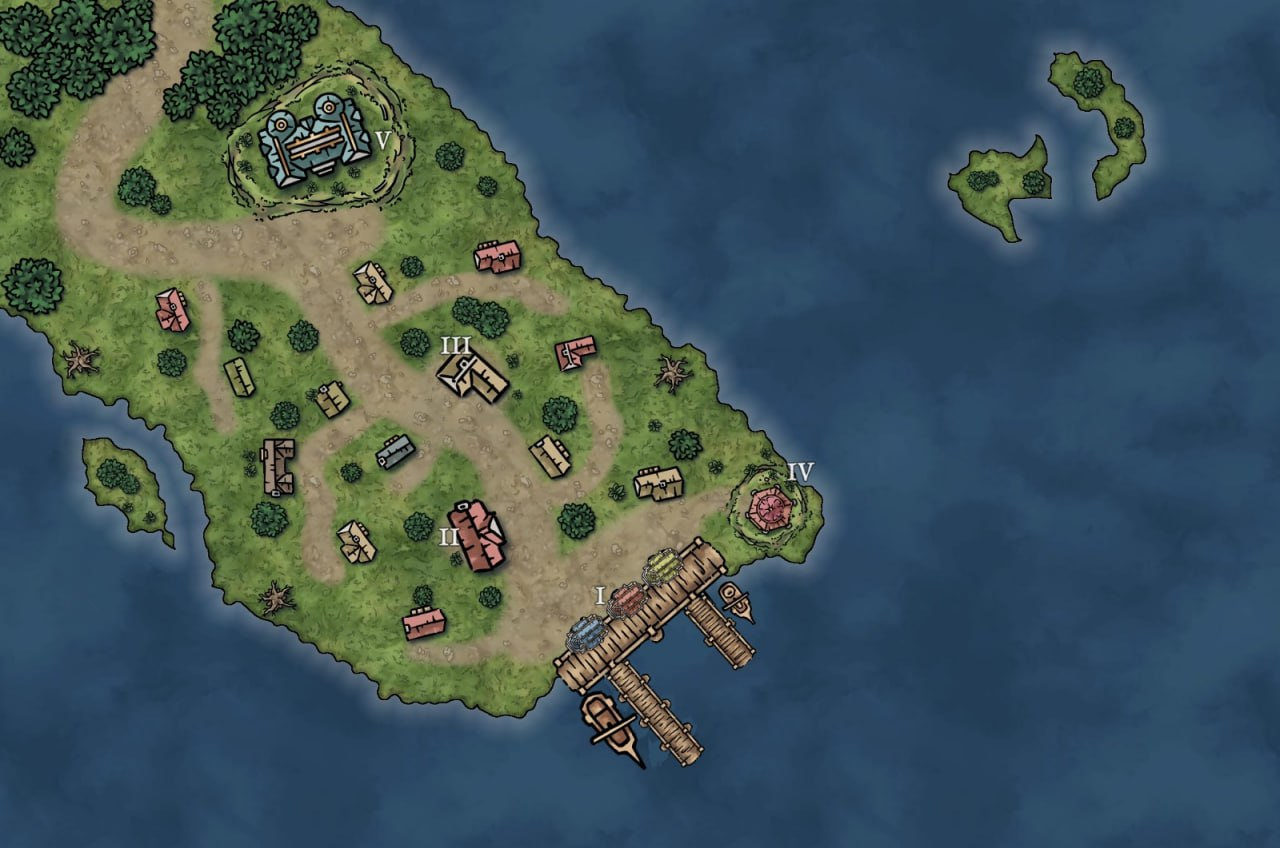
\includegraphics[width=9cm]{./mappe/mappa-middok.png}
\caption{La mappa di Middok}
\label{middok}
\end{figure}


Ci troviamo alla fine di una penisola dove si sviluppa il villaggio di Middok.
Il capitano Vitrovis offre vitto, alloggio e un passaggio in cambio di qualche giorno di lavoro sulla loro nave; il capitano sembra un uomo virtuoso, portano cibo e provviste alla persone del villaggio, con lo scopo di aiutare più che di guadagnare.
Ci si imbatte in tre bancarelle:
\begin{itemize}
  \item Giovane partenopeo mezzorco che vende pesce, il pesce normale è di qualità, quello "raro" probabilmente una truffa
  \item Ragazzo gentile armaiolo, aiuta il padre con la bottega, ci informa sull'affidabilità del vicino mezzorco e ci consiglia di andare dal borgomastro se cerchiamo qualche lavoro
  \item Ragazza halfling (Tamara) che vende strumenti per barca: bussole, quadranti, ecc.
\end{itemize}
Vitrovis litiga con un ragazzino che vuole salire con lui (10-14 anni), il ragazzino scappa tra la folla dopo che Felix lo ha strattonato. Il ragazzino è il figlio del borgomastro.

\subsection{Il borgomastro}
Verso la casa del borgomastro si vede che essa è molto più sfarzosa delle altre; un passante sostiene che non se la passino male, ma che il paese sia sceso di importanza rispetto a un tempo, quando era luogo di partenza e centro della vita dei mari. Il passante riporta che il borgomastro si occupa soprattutto della sua villa e dei nuovi avventurieri, come un normale borgomastro non troppo virtuoso né troppo prepotente.

Il borgomastro Vlaumack ci accoglie, parla della minaccia di temibili pirati avvistati lungo le coste; offre nave e aiuti per andare a respingerli. Il borgomastro risulta sospetto: offre una barca che pare più un relitto, sembra interessato a proteggere le sue ricchezze più che la sua popolazione, elogia gli avventurieri per convincerli a partire, è amico del mezzorco.
Puppis entra in bagno e ruba una saponetta (che è nuova e non rovinata), la domestica ripulisce subito il bagno dopo l'utilizzo.
Il borgomastro offre 15 monete d'oro a test in cambio dei tre pirati che si presume si aggirino in quelle acque (hanno taglie da 20 dobloni ognuno); Stone ha trattato per avere anche il sestante.

\subsection{La locanda}
La locanda è grande, con l'insegna storta; un po' di gente pranza ma non tanta. La vecchietta cordiale è madre del proprietario della locanda e amica di Vitrovis, non è troppo preoccupata per i pirati e indica Zonoi, la vecchia guardiana del faro, che potrebbe avere maggiori informazioni. Zonoi non ha visto pirati se non da bambina, ritiene che il borgomasto abbia ragione a temerli, ma non li ha effettivamente visti nelle vicinanze. Felix fa critico per riparare l'insegna della locanda che era storta, in cambio l'oste offre cena e letto per una notte (Stone dà 2 reals per compassione).

Viene pagato il pranzo per 2 reals; parlando con il proprietario della barca lo aggiorniamo su chi abbiamo incontrato. Gli avventurieri partiti con la nave del borgomastro sono stati depredati e ne è tornato solitamente uno per party.

A pranzo Felix sembra turbato, ansima con il battito accelerato e parla da solo ripetendo ``stai zitto"; Victor comincia a suonare armonica e ukulele per calmare la situazione, ma la gente si ammucchia e Felix si agita ed esce. Victor guadagna due monete per lo spettacolo ed esce per inseguire Felix, che è a pancia in giù steso per terra che dorme. Felix e Victor rientrano, Victor viene acclamato dalla folla.

\subsection{Il faro} Sulla via verso il faro Victor si sgancia dal gruppo e chiede al capitano Vitrovis se sia vera la questione dei pirati, egli riferisce di averli visti. La guardiana del faro vive lì da molti anni con un uccellino, impiegano molto tempo a salire le scale con la vecchietta. Parla di un'isola ``della Luna nascente", a una settimana di navigazione a Est del faro, a Nord - Est altro isolotto e a Nord - Ovest isola molto più abitata ma molto lontana (una decina di giorni di distanza). Zonoi ci regala una bussola. Grande partenza: Zonoi da piccola voleva fare la guardiana del faro da piccola, un tempo Middok era un luogo di grandi partenze. Tamara viene dal mare e si è fermata qua, l'armaiolo è venuto dalla terra. Stone chiede di essere successore del guardiano del faro, Zonoi spera che ci andrà qualcuno di bravo al suo posto.

\subsection{La notte alla Locanda}
Ritorniamo al porto e saliamo sulla barca per controllarla. È un po' più grande di una barca a vela, ha un piano di sotto ed è tutta un po' rovinata, ci sono due cannoni con palle e polvere da sparo; tutto è un po' rovinato; c'è qualche materasso e buchi tappati con assi di legno.

Chiediamo consiglio a Vitruivis, che sta parlando con Carlos (il proprietario della locanda); Vitruvis non è convinto ma dice che possiamo andare se abbiamo bisogno di soldi. Carlos si intromette e dice che i pirati sono temibili e che sembra che la situazione sia complessa, il borgomastro sembra avere molta paura (avendo più da rischiare).

\subsection{Il viaggio}
Il viaggio di mezza giornata, tre giorni di provviste ma dobbiamo restituire il sestante, verso Sud - Est.





\section{S2 - 06/08/2024}
Torniamo da Tamara, la mercante che commercia in articoli per la navigazione, e trattiamo il prezzo di un set di carte nautiche e un portacarte; nel mentre Puppis prende nel molo dei pezzi per fare una canna da pesca. Puppis sarà il cartografo del gruppo.

Il piano per catturare o uccidere i pirati è di fingere la resa per farci attaccare: possiamo far sventolare a Puppis o Victor un fazzoletto bianco, mentre gli altri membri dell'equipaggio sono nascosti e pronti ad attaccare. Dopo un momento di incertezza nella partenza ci ricordiamo che oltre a issare la vela è opportuno issare anche l'ancora e salpiamo verso Sud - Est: Puppis si apposta a osservare in cima all'albero maestro, Felix medita, Victor prepara i cannoni, ma nota che i cannoni sono rotti ed esclama insulti al borgomastro.

Nella stiva scopriamo essersi nascosto il figlio del borgomastro Fennop, un giovane di 14 anni che vuole combattere; gli diciamo di stare in silenzio nella stiva. Victor fa una prova ottima su navigazione e individua perfettamente le coordinate con il sestante. Individuiamo una nave, intimiamo a Fennop di andare in coperta, ma non collabora; Victor dice a Fennop di essere come la fatina dei denti, ma che stacca i denti ai bambini e Fennop va sotto coperta.

Puppis scorge una nave ad una distanza di circa 10km. Ci avviciniamo alla nave, Victor alza un braccio in segno di tregua e lancia un incantesimo per lasciare una scia di acqua rossa dietro di loro come fosse sangue. La nave si avvicina, un pirata sta reggendo il timone e gli altri due non sono visibili. Ora le due navi sono abbastanza vicine da parlare: Victor chiede aiuto ai pirati, che gli dicono che sono le persone più pericolose della zona. Su invito di Victor i pirati salgono sulla nave: Fennop sta per far saltare il piano, Victor prova ad addormentare i pirati ma fallisce. Tira fuori petali e sabbia per lanciare l'incantesimo sonno e i pirati giudicano il suo lato femminile.

I pirati vogliono perquisirci ma ci rifiutiamo, Felix toglie l'asse che collega le navi e comincia il combattimento.
Uno dei pirati esita guardando Fennop.

Inizia il combattimento che porta alla morte dei 3 pirati e al danneggiamento della nave fornita dal borgomastro a causa dell'urto con uno scoglio.

Esplorando la nave pirata troviamo 3 martelli da guerra da rivendere alla bancarella al molo, una caraffa d'oro del valore di 15 dobloni,  un reliquiario del valore di 10 dobloni, un anello del valore di 5 dobloni, un completo intimo femminile. Iniziamo a navigare verso Middok.

\section{S3 - 08/08/2024}
Dopo aver trasferito le ultime cose dal relitto alla nave pirata partiamo con rotta Nord-Ovest. Durante il viaggio Felix da di matto e attacca, apparentemente senza alcun motivo, Victor. Con un colpo di mazza ferrata e un secondo attacco da monaco Felix porta Victor a zero punti ferita lasciandolo in bilico fra la vita e la morte.

Puppis e Stone provano a contrastare la furia omicida di Felix che più viene attaccato più sembra aumentare la sua follia. Ad ogni turno Victor tira il dado per salvarsi dalla morte tuttavia i primi due tiri falliscono. Puppis prova a salvare Victor tirando su medicina ma con esito negativo, poi al secondo tentativo offre a Victor un successo nel tiro salvezza. In seguito Stone riuscirà a dare a Victor 2 tiri salvezza contro la morte stabilizzandolo privo di coscienza.

La furia omicida di Felix sembra placarsi dopo che Puppis lancia una "secchiata" di Rum in faccia a Felix. Stone e Puppis decidono di legarlo per scongiurare altri attacchi.

Quando Victor riprende coscienza recuperando 1 PF si alza per infilzare con la sua spada il petto di Felix ma fallisce il colpo. Stone e Puppis legano anche lui e riprendono la navigazione verso Middok.

Raggiungono il porto, ma una manovra sbagliata di Stone che si trova al timone fa si che venga distrutto il molo del porto di Middok. Mentre Stone e Puppis discutono con la folla che si è radunata per guardare il disastro del molo, Victor, legato, tenta una beffa crudele a Felix ma fallisce. Puppis interviene e lo convince a comportarsi con onore e smetterla di attaccare il suo compagno per vendetta. Victor accetta in segno della lealtà di Puppis che ha cercato di salvarlo quando era in fin di vita.

Sulla nave restano Felix legato e Fennop a controllare il prigioniero. Gli avventurieri scendono dalla nave e per superare l'imbarazzo del molo distrutto dalla manovra sbagliata Victor insulta tutti i cittadini presenti dicendo che in questa città sono degli incapaci e non sanno neanche costruire un molo decente e per scacciare dei pirati hanno dovuto chiamare dei forestieri. I cittadini lo guardano confusi, mentre Vitruivis, il capitano del mercantile, non si lascia ingannare dal bardo e guarda Victor in modo critico. Victor risponde strizzando l'occhio a Vitruivis.

\begin{DndComment}{Dal diario di Victor Vega}
Oggi quel pazzo di Felix quasi mi uccideva! Avevo capito alla locanda dell'Albatros che il ragazzo era tormentato ma non avrei mai pensato che potesse diventare un rischio per l'incolumità dei sui compagni. Devo tenerlo d'occhio, non voglio certo rischiare la vita per colpa di uno dei miei compagni. Puppis, che non ho ancora capito se sia una ragazza o un ragazzo, e Stone invece mi piacciono molto mi hanno aiutato nei momenti di difficoltà e nella battaglia contro i pirati si sono difese ..difesi.. bho... con coraggio e lealtà.
\end{DndComment}

\section{S3 - 09/08/2024}
Victor dopo aver ingannato la folla per la questione del molo distrutto diventa serio e dice a Stone e Puppis di dover fare una cosa. Sale a bordo per incontrare Fennop. Cerca di capire se sia realmente intenzionato a diventare un avventuriero e a rischiare la vita nonostante la sua giovane età. Poi gli chiede di mostrargli le sue armi e gli chiede il suo coltello da cucina rubato presumibilmente al madre. Infine dice a Fennop che cercherà di capire se suo padre è realmente cattivo con lui o esclusivamente protettivo. Se è cattivo gli promette che lo prenderà con se, senza tuttavia garantirgli protezione.

Terminato il colloqui con Fennop, Victor va da Felix legato all'albero maestro. Victor ha il coltello di Fennop in mano e sia avvicina a Felix guardandolo negli occhi. Felix si agita e cerca di allontanarsi per non essere ferito. In quel momento Puppis sale a bordo e interviene Victor gli intima di farsi li affari suoi. Victor si avvicina a Felix, alza il coltello e taglia le corte che legano Felix poi, voltandogli le spalle, gli dice che non può rischiare la propria vita per colpa di delle follie di un compagno. Infine gli dice "Ora se libero di andare dove vuoi ma sappi che non voglio rischiare la vita per colpa tua". Il gruppo discute per cercare di capire cosa tormenta Felix, il quale si limita a spiegare che questa follia è causata da un avvenimento del suo passato del quale non vuole parlare. Durante il prossimo viaggio probabilmente disarmeranno Felix anche se per essere letale non ha bisogno di armi. Felix, rendendosi conto del suo disaggio, si dimostra collaborativo ed è d'accordo nel consegnare le armi.

\section{S4 - 13/08/2024}
Scesi dalla nave salutiamo Vitrovis, che ci dice che gli abitanti della Luna nascente sono un po' restii a parlare con gli stranieri, hanno interessi per i loro affari e poco altro. Vitrovis ci avvisa che l'isola a Sud - Est è abitata da molti pirati e che i militari potrebbero avere altre taglie.

Chiediamo informazioni sul borgomastro, cercando di capire se voglia davvero il bene di suo figlio; a Vitrovis risulta che egli abbia provato a cercare il figlio nell'assenza e abbia mandato guardie alla taverna.

La caserma è una casa malridotta, più piccola della taverna. Delle guardie stanno giocando a carte, li informiamo che abbiamo i cadaveri dei pirati nella nave; la guardia sembra svogliata e dice che dobbiamo portare i cadaveri al carcere. Victor lancia Charme su persone alla guardia e la convince a venire a vedere i cadaveri dei pirati direttamente sulla nave. Ci vengono assegnate le taglie sui pirati (18 scudi per tutti e tre) e convinciamo la guardia ad accompagnarci dal borgomastro per testimoniare la nostra missione.

Victor e il borgomastro litigano; Puppies si fa il bagno nel mentre. Stone fa firmare al borgomastro un contratto per pareggiare i conti in cambio di 15 dobloni in meno dalla paga. Si accende una lite con il borgomastro, Felix e Victor lo minacciano, il borgomastro se ne va indignato. Il borgomastro metta una taglia su di noi e siamo ufficialmente ricercati.

\begin{DndComment}{Dal diario di Stone}
Lo so che noi Tortuga amiamo l'avventura, lo so. Però dopotutto una vita tranquilla fra i campi... Non mi aspettavo sarebbe stato così difficile: la mia compagnia ha ucciso tre persone di cui non conoscevamo la storia, magari erano brave persone e io ho contribuito alla loro morte. Ho avuto un momento di debolezza, ma devo tenere alto il nome del Tortuga e onorare il coraggio della mia famiglia! Proverò a fare quest'ultimo viaggio verso l'isola della Luna nascente...
\end{DndComment}

Quando torniamo alla nave 2 guardie ci aspettano per arrestarci, ma fra incantesimi e qualche colpo riusciamo a salpare.

\begin{DndComment}{Dal diario di Victor Vega}
Il borgomastro di Middok non mi piace. Tiene i suoi cittadini in povertà e lui vive nell'agiatezza. Gli avrei tagliato volentieri la gola se non fosse stato per il piccolo Fennop al quale mi sono affezionato. Prima o poi riuscirò a scatenare una rivolta del popolo di Middok e a spodestare il Borgomastro a favore di una persona di maggior valore.
\end{DndComment}


\chapter{NPC}

\subparagraph{Fennop} Figlio quattordicenne del borgomastro Vlaumak. Ha l'ambizione di diventare un marinaio, forse un pirata. Non sa nuotare.

\subparagraph{Tamara} Commerciante di Middok. Vende articoli per la navigazione. Zonoi ha detto che Tamara viene dal mare

\subparagraph{Vitruvis} Capitano di una nave che commerciale che commercia prodotti con il villaggio di Middok. Sembra una brava persona e lo fa anche per sostentare gli abitanti della città.

\subparagraph{Vlaumak} Borgomastro della città di Middok. La sua villa è molto lussuosa a differenza di tutte le case del villaggio.

\subparagraph{Zonoi} Anziana guardiana del faro di Middok.
\end{document}